\documentclass{article}
\usepackage[UTF8]{ctex}
\usepackage{geometry}
\usepackage{natbib}
\geometry{left=3.18cm,right=3.18cm,top=2.54cm,bottom=2.54cm}
\usepackage{float}
\usepackage{graphicx}
\pagestyle{plain}	
\usepackage{setspace}
\usepackage{caption2}
\usepackage{datetime} %日期
\renewcommand{\today}{\number\year 年 \number\month 月 \number\day 日}
\renewcommand{\captionlabelfont}{\small}
\renewcommand{\captionfont}{\small}
\begin{document}

\begin{figure}
    \centering
    
\includegraphics[width=8cm]{upc.png}

    \label{figupc}
\end{figure}

	\begin{center}
		\quad \\
		\quad \\
		\heiti \fontsize{45}{17} \quad \quad \quad 
		\vskip 1.5cm
		\heiti \zihao{2} 《计算科学导论》课程总结报告
	\end{center}
	\vskip 2.0cm
		
	\begin{quotation}
% 	\begin{center}
		\doublespacing
		
        \zihao{4}\par\setlength\parindent{7em}
		\quad 

		学生姓名:\underline{\qquad  李弟诚 \qquad \qquad}

		学\hspace{0.61cm} 号:\underline{\qquad 1907010105\qquad}
		
		专业班级:\underline{\qquad 计科1901 \qquad  }
		
        学\hspace{0.61cm} 院:\underline{计算机科学与技术学院}
% 	\end{center}
		\vskip 2cm
		\centering
		\begin{table}[h]
            \centering 
            \zihao{4}
            \begin{tabular}{|c|c|c|c|c|c|c|}
            % 这里的rl 与表格对应可以看到,姓名是r,右对齐的;学号是l,左对齐的;若想居中,使用c关键字。
                \hline
                课程认识 & 问题思 考 & 格式规范  & IT工具  & Latex附加  & 总分 & 评阅教师 \\
                30\% & 30\% & 20\% & 20\% & 10\% &  &  \\
                \hline
                 & & & & & &\\
                & & & & & &\\
                \hline
            \end{tabular}
        \end{table}
		\vskip 2cm
		\today
	\end{quotation}

\thispagestyle{empty}
\newpage
\setcounter{page}{1}
% 在这之前是封面,在这之后是正文

\section{引言}
一个学期的计算机导论课已经告一段落了。上这门课,不仅让我从最初的计算机小白变成对计算机这门课程的框架有大体认识的人,还让我在课堂上开阔了视野,收获了知识。孙运雷老师清晰的教学思路,合理的教学安排让我在这堂课上受益颇丰,对我以后的学习和生活也有至关重要的影响。\par
从1946年冯诺依曼的ENIAC问世到现在计算机走进千家万户,计算机经过半个多世纪的发展,四次改革终于达到了现在这个水平。现如今,计算机已经成为人们生活的必需品,前景良好。但我国在计算机的发展上落后了一段时间,目前我国计算机人才仍然短缺,与美国等发达国家也有不小的差距。身为计算机专业的学生,学好这门课成为了我们肩上的重任。而孙老师讲授的这门计算机导论课,赵致琢老先生写的这本《 计算科学导论》为我们提供了重要的指引。
\section{对计算科学导论这门课程的认识、体会}
赵致琢老先生编纂的这本《 计算科学导论》为我们指引了学习这门课的方向。这本书介绍的计算机的基本概念和基本知识,计算科学的意义、内容和方法等都是身为计算机专业的学生应该掌握的。这本书结构清晰,在开头便向我们介绍了计算机的历史,名词的来源,增强了我对计算机和计算机专业的认识。更重要的是,这本书通过向我们讲述科学哲学与科学方法论、一般的科学思想方法、计算科学初学者的正确选择等,告诉了我们拥有一种认识与实践的方法学概念会让我们事半功倍,指明了我们学习这门课程该走的路;通过向我们介绍计算科学的基本概念和基本知识,开拓了我们的视野,将像并行计算机、通道与并行计算,计算机网络与通信,计算机图形学与图像处理,逻辑与人工智能到数据处理与演化计,计算机科学与技术一级学科等领域内的一些重要的基本概念带进了我们的世界;通过向我们介绍计算科学的意义,内容和方法,讲述如何学习计算科学、健康成长,不仅让我了解到计算机科学与技术学科的定义、基本问题、学科方法论、学科发展的潮流与未来发展方向以及组织结构及其演变等问题,还让我了解到在学校培养计算机科学与技术一级学科创新人才与高素质专业技术开发人才的过程中如何使我们正确地认识和学好计算机科学与技术学科。\par


\subsection{学科方法论}
在本书的第一章就给出了学科方法论的简介。学科方法论由科学的方法论与一个具体学科相结合的产物,属于科学哲学层面和该学科科学哲学的研究范畴。它是要研究学科中不同学科领域和方向内一类科学概念、原理、方法、技术特性,相互之间更为抽象的共同特性、特征、相互之间的关系、以及使用这些概念、原理、方法、技术的更一般化的原则、原理、方法、技术及其合理性问题。例如计算机学科方法论就是对计算机领域认识和实践过程中的一般方法、性质、特点、内在联系和变化规律进行的系统研究和理论总结.\par
如果把学科知识体中的内容比之为 “鱼”,那么学科方法课程就是获得鱼的方法及工具。学科方法论从学科的科学问题、学科的抽象、理论和设计三个过程以及学科的核心概念、数学方法和系统科学方法等方面出发,深刻地揭示了学科的本质,有助于我们对计算学科的认识。而学科建设首先是建立在对学科的认知基础上的。因此,它有助于学科的建设和人才培养,更有助于总结和提升学科积累的各种方法与经验.\citep{ll}\par
孙老师的这门课程使我接触到了学科方法论,让我懂得了了解一个学科的方法论对加速自己的研究进程,取得成果有很大作用,对我日后进行研究学习指出了关键点。在我看来,计算机导论这门课难道不就是学习计算机学科的方法论的重要组成部分么?\par

\subsection{科学的思想方法}
在《计算科学导论》第一章介绍了一般的科学思想方法,科学的思想方法就是帮助我们用更一般的思想方法或工作原则来较好地解决问题的方法。我们所倡导的一般的科学思想方法概括起来就是一个科学的认识、一套科学的方法、一个科学的程序。善于使用正确的科学思想方法,能让我们迅速了解和进入一个可能完全不熟悉的领域,能让我们更好更快的解决问题。\par
我在以往的学习过程中,并没有,甚至根本没有去想一套科学的思想方法,这造成我上课效率低,课后要比别人多花很多功夫才能赶上,老师上课带我们去了解的科学的思想方法让我不由地去反思自己,什么是科学的思想方法,怎么样才能善于使用科学的思想方法?这正是当下我们应该去思考的问题。同时,了解一些经典的计算科学方法对我们也大有裨益,比如公理化方法,演化方法。
\par
%\begin{table}[h]
   % \centering
   % \caption{这是科学系的花名册}
%\begin{tabular}{rl}
% 这里的rl 与表格对应可以看到,姓名是r,右对齐的;学号是l,左对齐的;若想居中,使用c关键字。
  %  \hline
  %    姓名 & 学号 \\
    %   \hline
    %   张三 & 190704xxxx+++ \\ 
     %  李四 & 190704yyyy \\
      % 王二五 & 190704zzzz\\
      % \hline
  % \end{tabular}
     %  \label{table1}
  % \end{table}

\par

\section{进一步的思考}
通过查阅资料与文献,我和我的队友也终于对云桌面有了一个初步的认识,在我们将我们的成果进行汇报演讲后,经过孙云雷老师和同学们的当堂指正和补充后,我发现仍然有很多问题像云数据的安全,使用云桌面是否经济等问题还在我的认知范围之外。演讲后,我通过进一步搜寻资料,查阅文献,并将最后的结果在此汇报。\par


\subsection{云桌面简介}\par
云桌面就是将计算机的桌面进行虚拟化,以达到桌面使用的安全性和灵活性。用户可以通过任何设备,在任何地点,任何时间访问在网络上的属于用户自己的桌面系统。
\subsection{云桌面的发展史}\par
云桌面的发展大致分为五个时代。第一个时代为无盘工作站时代,早期PC 机硬盘价格昂贵,随着无盘技术的出现,人们统一使用服务器分配的共享存储。随后是硬盘克隆与写保护时代,进入21世纪后,人们开始思考如何为整间教室的数十台电脑安装统一操作系统、应用软件,以诺顿为代表厂商提供了网络克隆的解决方案。管理人员可以选择任意一台电脑作为标准机,通过网络(广播)克隆到其他所有的电脑中,实现批量克隆式交付。硬件级或系统软件级实现写保护,重启则还原。防止系统遭受破坏性的修改。然后就是终端远程桌面时代,微软在推出Windows 2000 Server 时提供了 Terminal Service 对RDP ( 远程桌面协议 ), RDP 则可以将用户的会话传输到远程的客户机上,安装RDP 的客户端,连接到远程的桌面。这种情况下用户实际上使用的是两个桌面,一个桌面在窗口中也就是我们今天所说的虚拟桌面,一个是自己本机的桌面。第四个时代是虚拟桌面时代,在纯软件全虚拟机技术越来越成熟的同时,Intel 、AMD 两家CPU 制造商在自己的处理器加入了虚拟化指令从CPU内核级提供了虚拟化的支持。管理人员可以在一台甚至一组集群服务器上创建大量的虚拟机,为每一个用户都分配一台虚拟机,用户所使用的虚拟桌面实际是服务器上某一台虚拟机的桌面,而不是服务器上某一个会话的桌面。虚拟机与虚拟机之间是隔离的,有着各自的地址空间。从根本上杜绝用户间访问冲突。这种模式也就我们传统意义称为的VDI ,VDI 的基本模型至今仍在延用。但是受到现有技术的瓶劲,虚拟机在高帧视频、图形图像处理方面的表现仍然不佳。因此国内更多厂商更愿意采用VOI 架构,VOI 无需在服务器创建运行虚拟机,仅需创建和提供一组虚拟磁盘,操作系统与应用软件都存放在虚拟磁盘中,所有用户可以共用一组虚拟磁盘来实现桌面交付,在快速统一交付系统与应用同时,VOI 能实现用户数据的个性化与外设、复杂硬件环境的兼容支持。并在高帧视频、图形图像处理方面的表现极佳。最后就是我们所提到的云桌面时代,随着计算机硬件性能与互联网传输速度的几何级提高,使得虚拟桌面的远程低损交付可为可能,用户可以根据自己需求租用(或免费申请)云主机或云存储用于工作和业务运营,这种服务模式被统称为“公有云” ,在2014年初云桌面 NGD 的理论被提出。

\subsection{云桌面的价值}\par
在传统桌面模式下,IT管理部门面临的挑战有桌面不统一,维护效率低,数据不安全,资源利用率低等问题。但是云桌面的使用很好的解决了上述问题,云桌面的好处如下
\begin{itemize}
	\item [1) ] 集中部署,减少维护提升桌面服务水平,维护便捷。
桌面云改变了过去分散、独立的桌面系统环境,通过集中管理,IT人员在数据中心就可以完成所有的管理维护工作,80\%的维护工作将自动完成,包括软件下发、升级补丁、安全更新等等,大大减少了大量的维护工作量。    
	\item [2)]
	远程托管,数据隔离。桌面云的用户桌面环境都是托管在企业的数据中心,本地终端只是一个显示设备而已。即便用户在桌面系统中保存了数据,该数据也仍然是在企业数据中心,而没有在用户的终端设备上保存任何副本。通过这样的数据隔离措施,企业能够有效的保证数据不被违规带出企业,保障了数据安全。 
	\item [3)]
	一个窗口,多个桌面。满足多业务处理要求在一些特殊企业工作环境中,员工往往需要同时用到多个桌面系统(一人多台PC),桌面云提供的托管桌面系统可以让用户在一个浏览器界面中,同时访问不同的后台桌面系统,并可以在不同系统间灵活切换。这样既满足了员工处理多个不同业务的需要,提升了员工工作效率,减少了空间占用,节约了投资。 
	\item [4)]
	远程接入。桌面云的托管桌面支持使用各种终端设备接入,而网络访问的方式为企业用户提供了非常灵活的工作处理能力,只要有网络的地方,员工都可以通过网络进入到企业的办公环境来处理工作。这种方式为企业提供了移动办公的能力。
	\item [5)]
	集中存储,灾难恢复快。桌面云的数据都是集中存储在企业数据中心,因此,企业就能够轻松的实现在不同站点间的数据复制,让桌面系统融入整体企业IT容灾体系中,构成一个完整的容灾体系。当灾难发生的时候,可以迅速恢复所有托管桌面,保证完全恢复业务的处理能力。实现了对桌面及应用的集中管理和按需交付,能够为各行业中各类型企业提供软硬一体化的交付方案。
;\end{itemize}

\subsection{云桌面的技术实现}\par
云桌面是云计算的一种应用模型,用户端可以通过输入输出操作控制在云端的虚拟机,从而获取云中的各类池化资源,同时把云端的虚拟机桌面视图呈现在用户端,其用户体验类似于微软Windows操作系统里的远程桌面。但云桌面的技术原理与远程桌面大相径庭。首先,用户通过普通桌面电脑、笔记本,平板电脑等客户端发起请求,连接到会话管理中心,会话管理中心是与服务器端一致的虚拟化集中管理工具,为服务器与桌面环境提供统一的管理平台:其次,会话管理中心对用户进行身份验证:最后,用户通过身份验证后,进入后台云数据中心,从虚拟机资源池中通过策略划拨一台桌面环境虚拟机,无缝地登录到虚拟桌面。随着虚拟桌面的使用完毕,云端的桌面环境可依据相应的管理策略释放已占用的资源,让资源回归云数据中心资源池。\citep{cc}
    \begin{figure}[H]
	\centering
	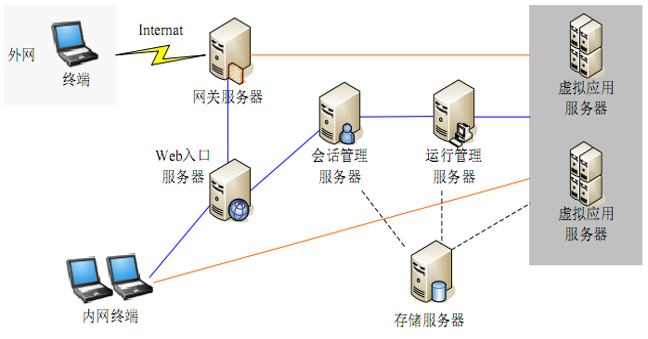
\includegraphics[width=8cm]{222.png}
	\label{figupc}
	
\end{figure}
\subsection{云桌面的安全问题}\par
云桌面作为云计算的内容之一,自然会存在与云计算相似的安全问题,安全问题也是阻碍云计算被广泛采用的最大障碍之一。很多商业和研究组织也都不愿完全信任云计算将数字资产转移给第三方服务提供商。\citep{bb}
    \begin{figure}[H]
	\centering
	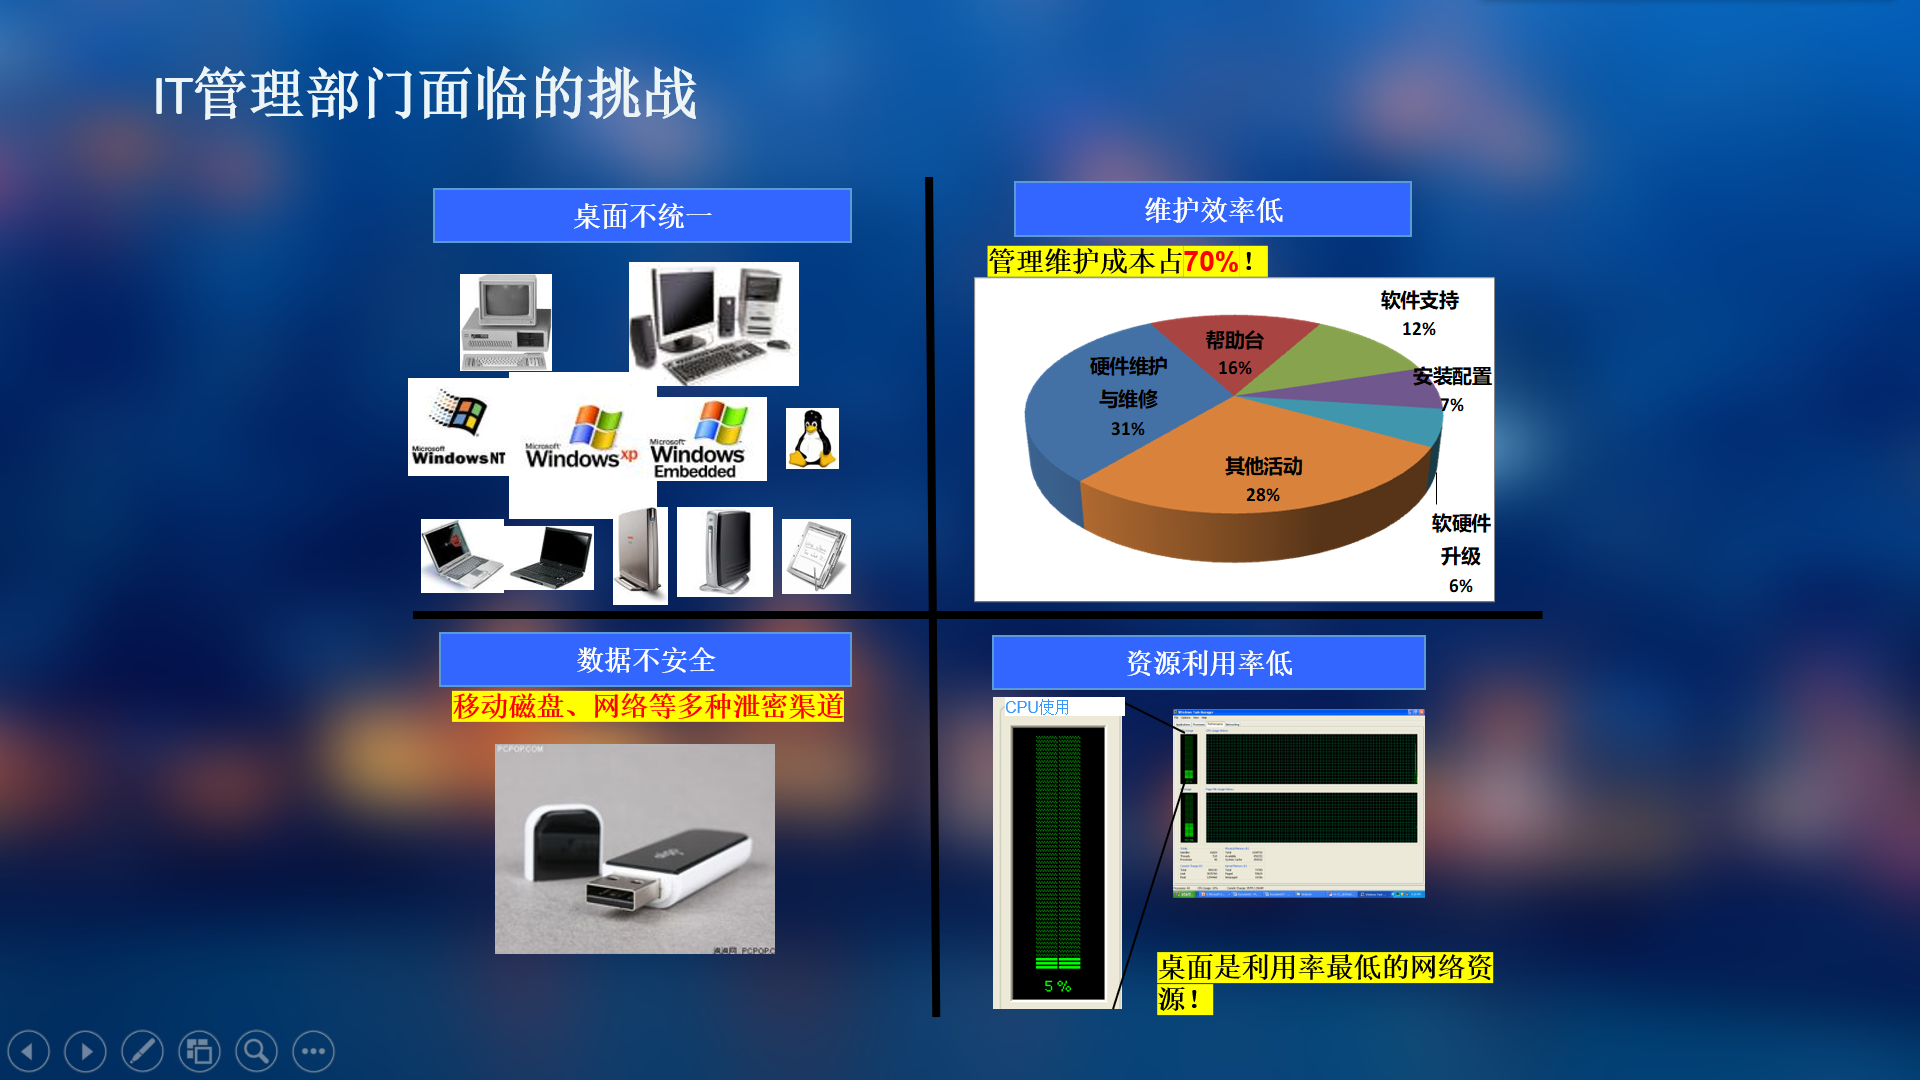
\includegraphics[width=8cm]{333.png}
	\label{figupc}
	
\end{figure}
因为在云桌面模式下,用户数据在用户使用完虚拟桌面后会自动回归和储存在云数据中心资源池,所以数据中心都保存有大量的私密数据, 这些数据往往涉及到用户的隐私。所以在此模式下, 使用云桌面面临着几个方面的问题:一是如何确保相关数据在网络传输过程中严格加密不被窃取; 二是如何保证云计算服务商在得到数据时不将相关数据泄露出去; 三是在云计算服务商处存储时, 如何保证访问用户经过严格的权限认证并且是合法的数据访问,并保证用户在任何时候都可以安全访问到自身的数据。针对这些问题,有以下四个方面的解决方案:
\begin{itemize}
	\item [1) ]
	数据加密\\
  	 加密技术是网络安全中一个非常重要的安全技术,数据加密是利用技术手段把要传输的重要的数据变为密文(加密)进行传送,到达接收端后再用相同或不同的手段对密文进行还原(解密。在\citep{dd}中提出了一种将对称加密与非对称加密相结合的云计算数据加密安全策略,这样做可以规避非对称加密数据效率低的弊端,还通过对密匙的非对称加密操作提高了用户数据的安全性
	
	\item [2) ]安全存储\\
	在实际应用中,网络中数据的存储是非常重要的环节,其中包括数据的存储位置、数据的相互隔离、数据的灾难恢复等,在云计算模式下,数据存储资源处于共享的环境下,即使有数据加密的技术的加入,云计算服务提供商是否能够保证数据之间的有效隔离也是一个非常重要的问题:另外,还需要做好备份措施,以防止出现各种网络和系统故障和宕机时,用户的数据被破坏,造成重大损失。
	
	\item [3) ]安全认证\\
	安全认证可通过单点登录认证、强制用户认证、代理、协同认证、资源认证、不同安全域之间的认证或者不同认证方式相结合的方式,其中很多用户是通过结合强制用户认证和单点用户认证的方式来允许用户进入云应用的认证,用户只需登陆一次进入整个web应用,从而可以有效的避免用户在使用自己的服务时将密码泄漏给第三方。
	
    \item [4) ]以集中的安全服务中心应对无边界的安全防护\\
    和传统的安全建设模型强调边界防护不同,存储计算等资源的高度整合,使得用户在申请云计算服务时,只能实现基于逻辑的划分隔离,不存在物理上的安全边界,在这种情况下,已经不可能基于用户或用户类型进行流量的汇聚并部署独立的安全系统,因此,安全服务部署应该从原来的基于各子系统的安全防护,转移到基于整个云计算网络的安全防护,建设集中的安全服务中心。
\end{itemize}\par
在此之外,云桌面中的VDI架构也能很好地解决安全问题。\citep{ee}因为是单纯的后端计算,数据从产生开始就在服务器上,能做到数据不落地,安全性很高。云桌面体系的办公环境下,为进一步满足特定用户对办公数据安全的需求,在不改变用户使用习惯的前提下,也可将用户桌面与用户办公数据隔离管理,在享用云桌面办公带来的便利的同时,提高数据安全的管理及容灾。
\subsection{云桌面的前景}\par
随着云计算快速发展,云桌面的产品以变得越来越成熟的它的应用也变得越来越广泛学校、企业办公、医院信息化建设以及培训中心等各行各业都能看到云桌面的身影,而未来的云桌面发展趋势会有以下几个方面的发展:
\begin{itemize}
	\item [1) ]桌面连接的多样化,现在大多数的云桌面连接方式都是比较单一的,比如呢用的是Linux底层的云桌面只支持X86架构的云终端不支持其他架构的云终端或者即使支持也达不到好的体验效果,未来的云桌面应该是不管是windows还是linux的云桌都可以通过云终端、PC和手机、平板电脑等硬件进行连接而不影响使用体验的。
	\item [2) ]一个平台多种协议,即根据不同的用户环境和应用需求在同一个平台部署多种协议来解决一个部门不同的办公需求,双协议模式可以很好的实现一个平台部署,统一管理,统一调度,大大减少了用户的设备、人员投入,减轻了运维负担对于那些大中型企业和高校等复杂应用的环境是一个很好的解决方案的。
	\item [3) ]混合云是首选,混合云:就是将私有云和公有云如何有效的进行搭配,不仅仅是简单的物理结构的连接,而是从更深层次的应用出发,结合用户需求,达到1+1大于2的效果, 在这一方面国内厂商禹龙云已做出了成功的混合云解决方案。
	\item [4) ]真正的实现移动办公,就是不管在哪里都可以通过云终端、手机平板以及PC等硬件来连接云端服务器实现移动办公而不影响性能体验,而现在很多说的移动办公都是要在同一个局域网环境下的移动办公即使有些不在同一个局域网可以连接但它的体验效果却不是很理想的。
\end{itemize}\par	
	如今时云计算快速发展的时代,是一个开放共赢的时代,作为云计算一个典型应用的云桌面随着技术的变革将会给我们提供更开方、更安全、更稳定和更便捷的用户体验。
	
	
\section{总结}	
转眼间计算科学导论这门课程就要结束了,我也从这门课当中受益不少。虽然在这本书的引言中,作者说这本书的内容不是大一学习的重点,但在我看来,这本书与我们而言,是一个方向,是一座灯塔,优秀的教材加上老师正确明朗的指引,让这门课的内容更加丰厚。在学习这门课程时,我对书中知识的内涵并不是很清楚,但是我必会在日后的学习中逐步去理解!这门课程虽然结束了,但是这门课对我的指引将会一直伴随着我接下来的学习。\par
孙老师给我们布置的分组演讲的作业,也让我收益颇丰。我在准备过程中加深了自己对云这一概念的了解,增长了我的见闻。我在今后也会像这样不断增长我的知识库,终有一天能为国家的计算机领域发展做出贡献!\par

\section{附录}
\begin{itemize}
    \item Github网址:https://bskingdom.github.io/bsentrance/
    \begin{figure}[H]
    	\centering
    	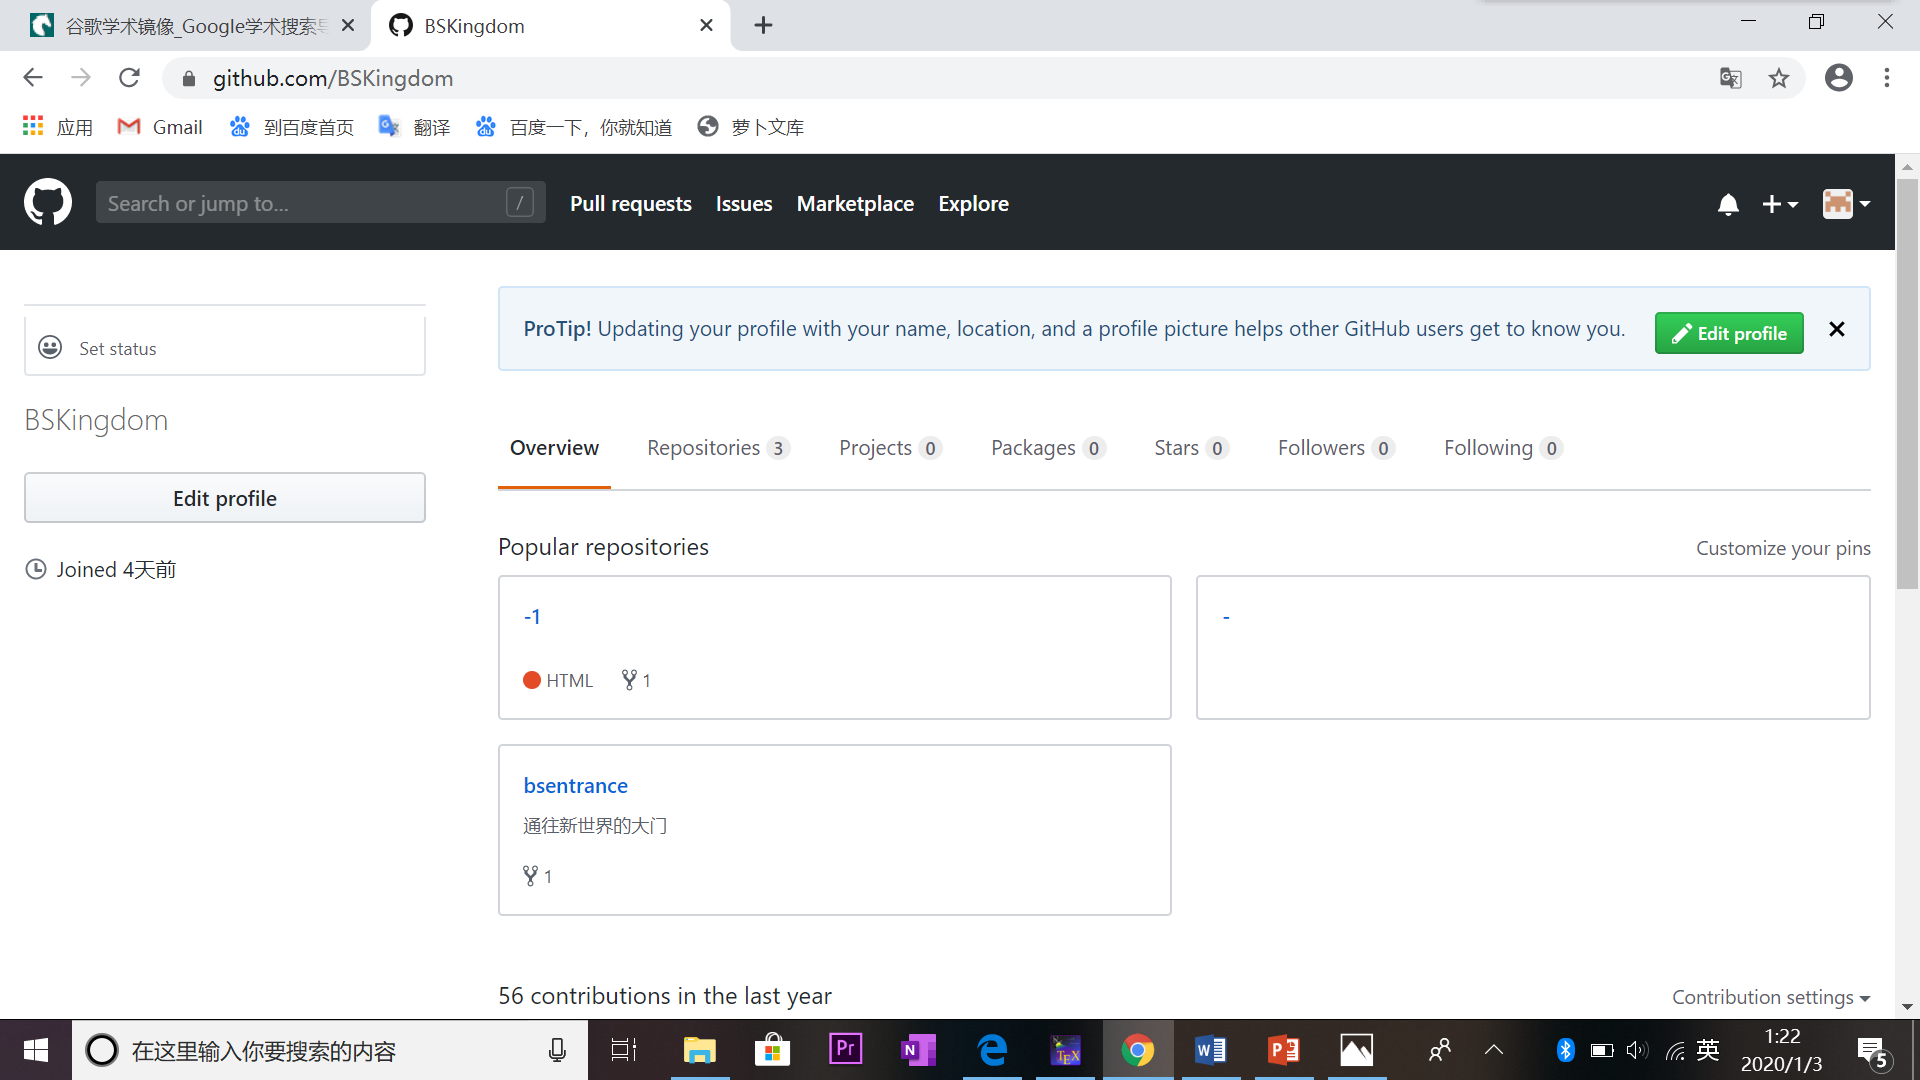
\includegraphics[width=10cm]{2020-01-03 (1).png}
    	\label{figupc}
    	
    \end{figure}
    
    \item     \begin{figure}[H]
    	\centering
    	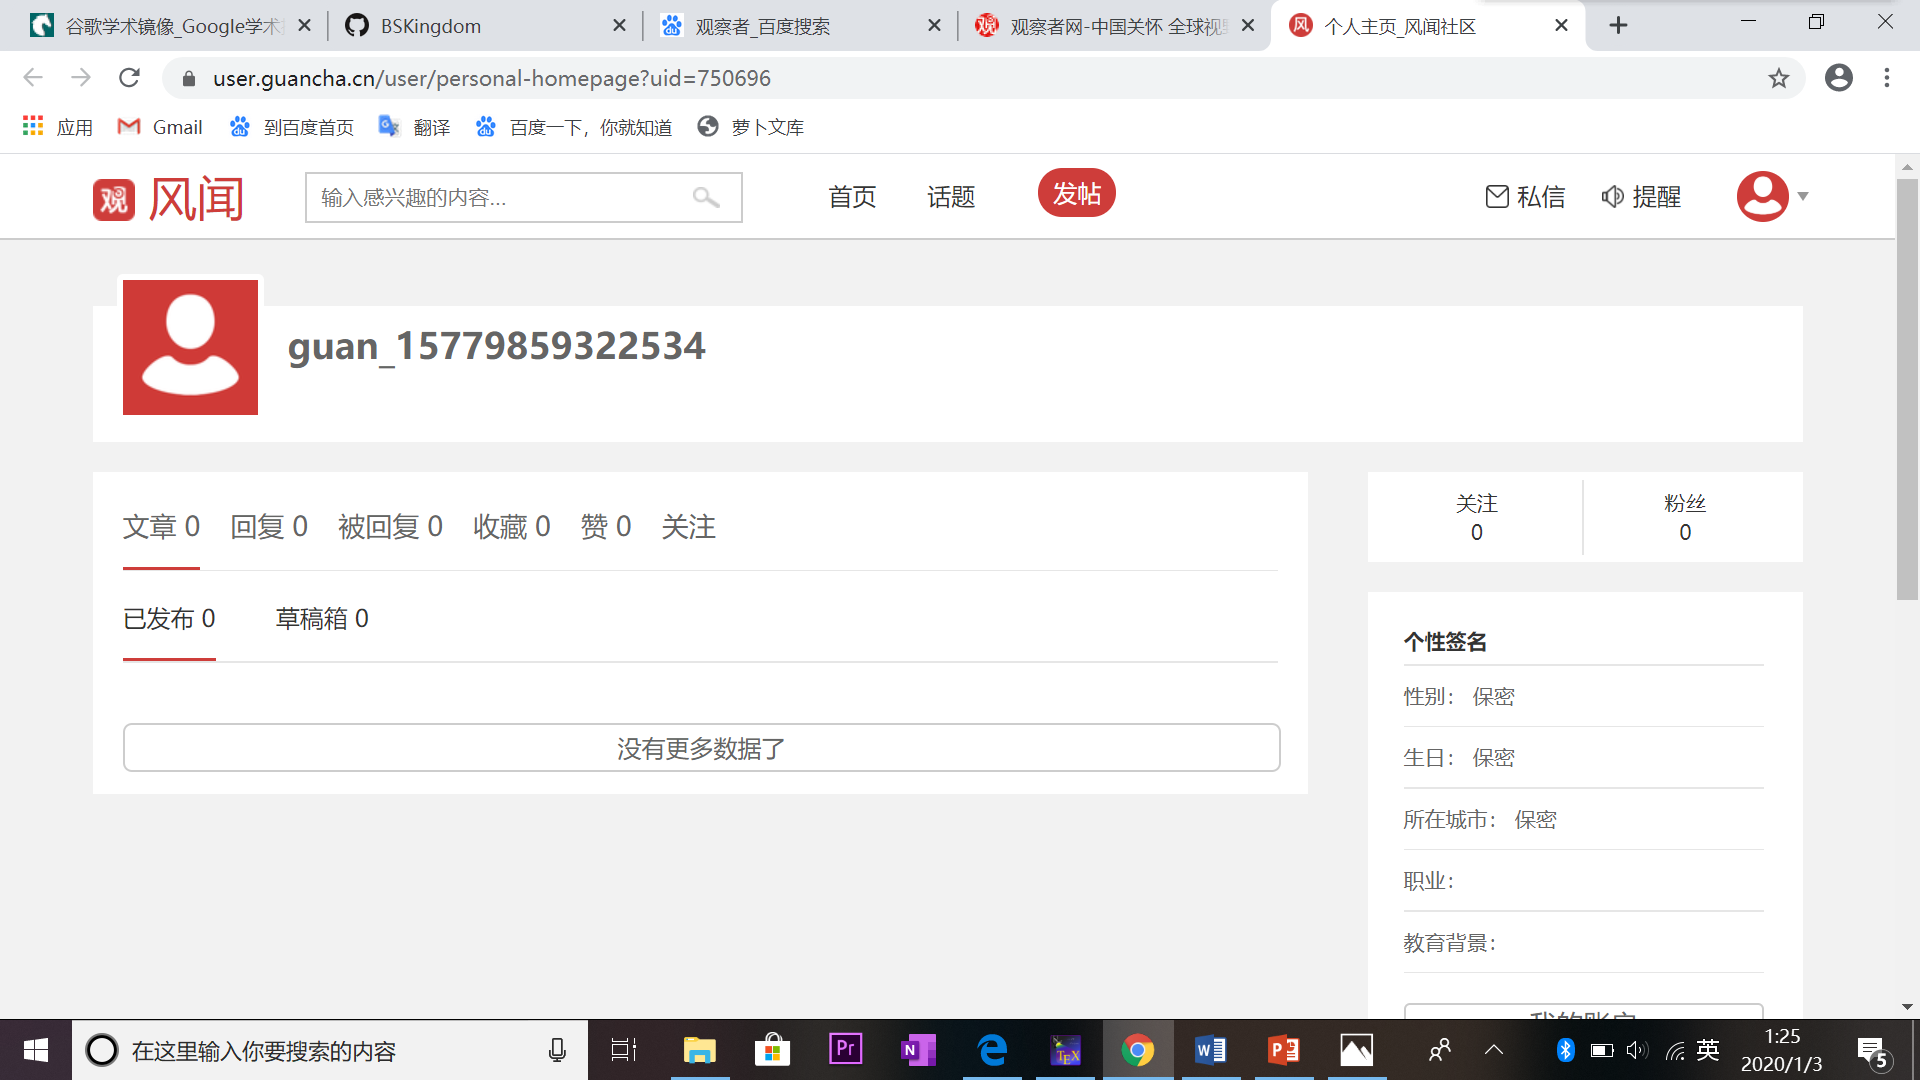
\includegraphics[width=10cm]{2020-01-03 (2).png}
    	\label{figupc}
    	
    \end{figure}
    \begin{figure}[H]
	\centering
	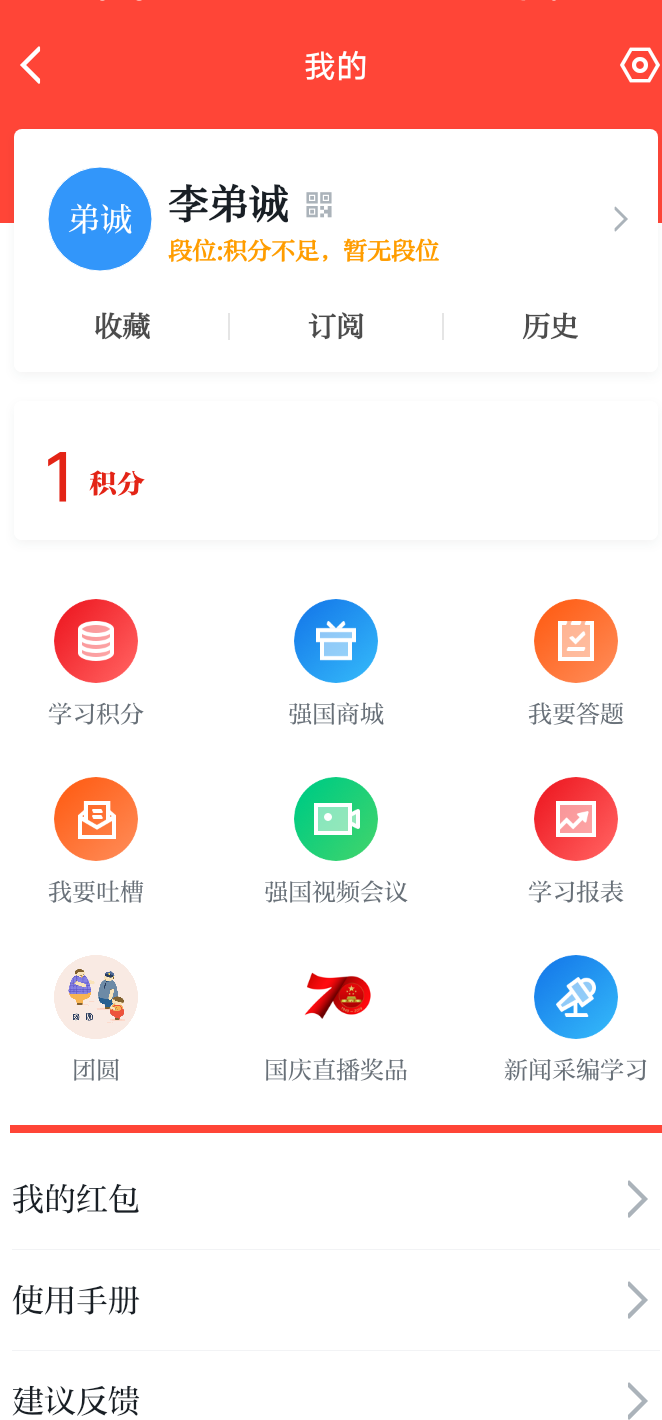
\includegraphics[width=6cm]{Screenshot_2020_0103_013207.png}
	\label{figupc}
	
\end{figure}
    \begin{figure}[H]
	\centering
	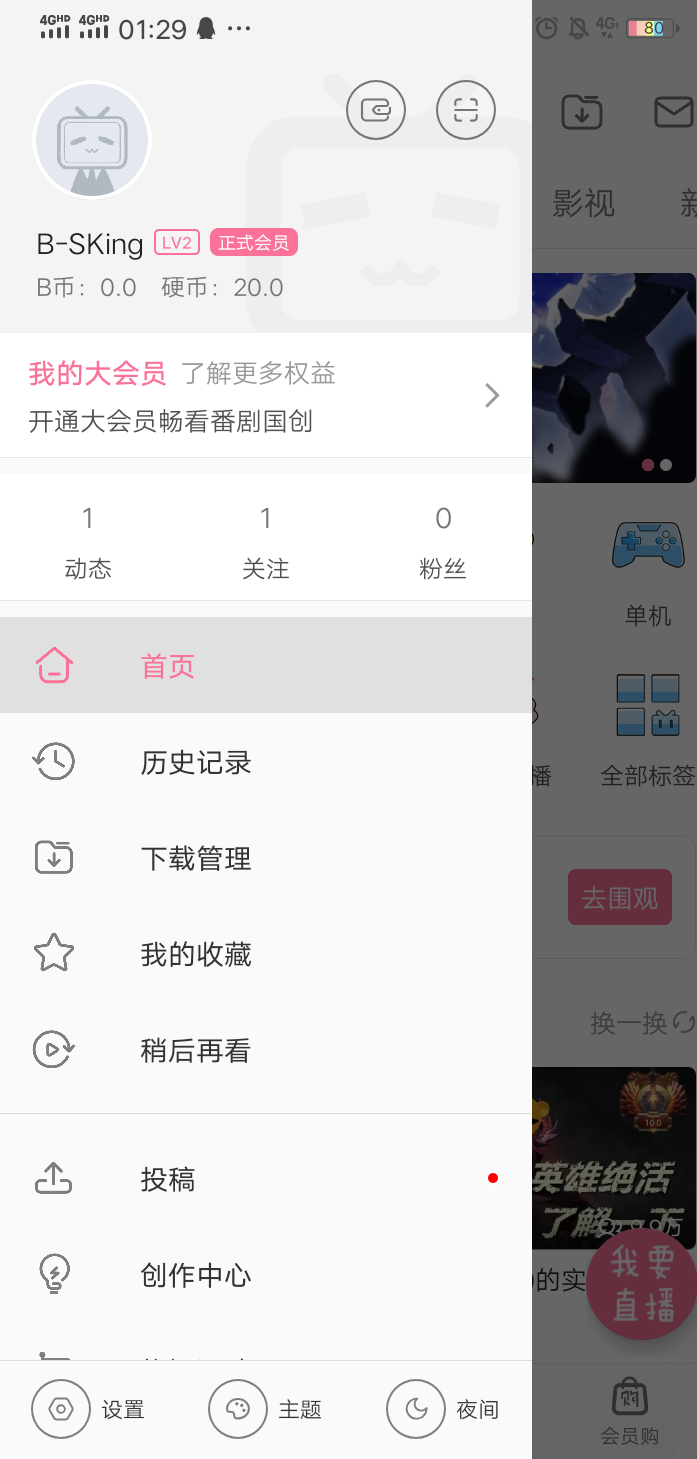
\includegraphics[width=6cm]{Screenshot_2020_0103_012920.png}
	\label{figupc}
	
\end{figure}
    \item 注册CSDN:https://me.csdn.net/BSKingdom 
    博客园网址:https://home.cnblogs.com/u/1914427/  \begin{figure}[H]
    	\centering
    	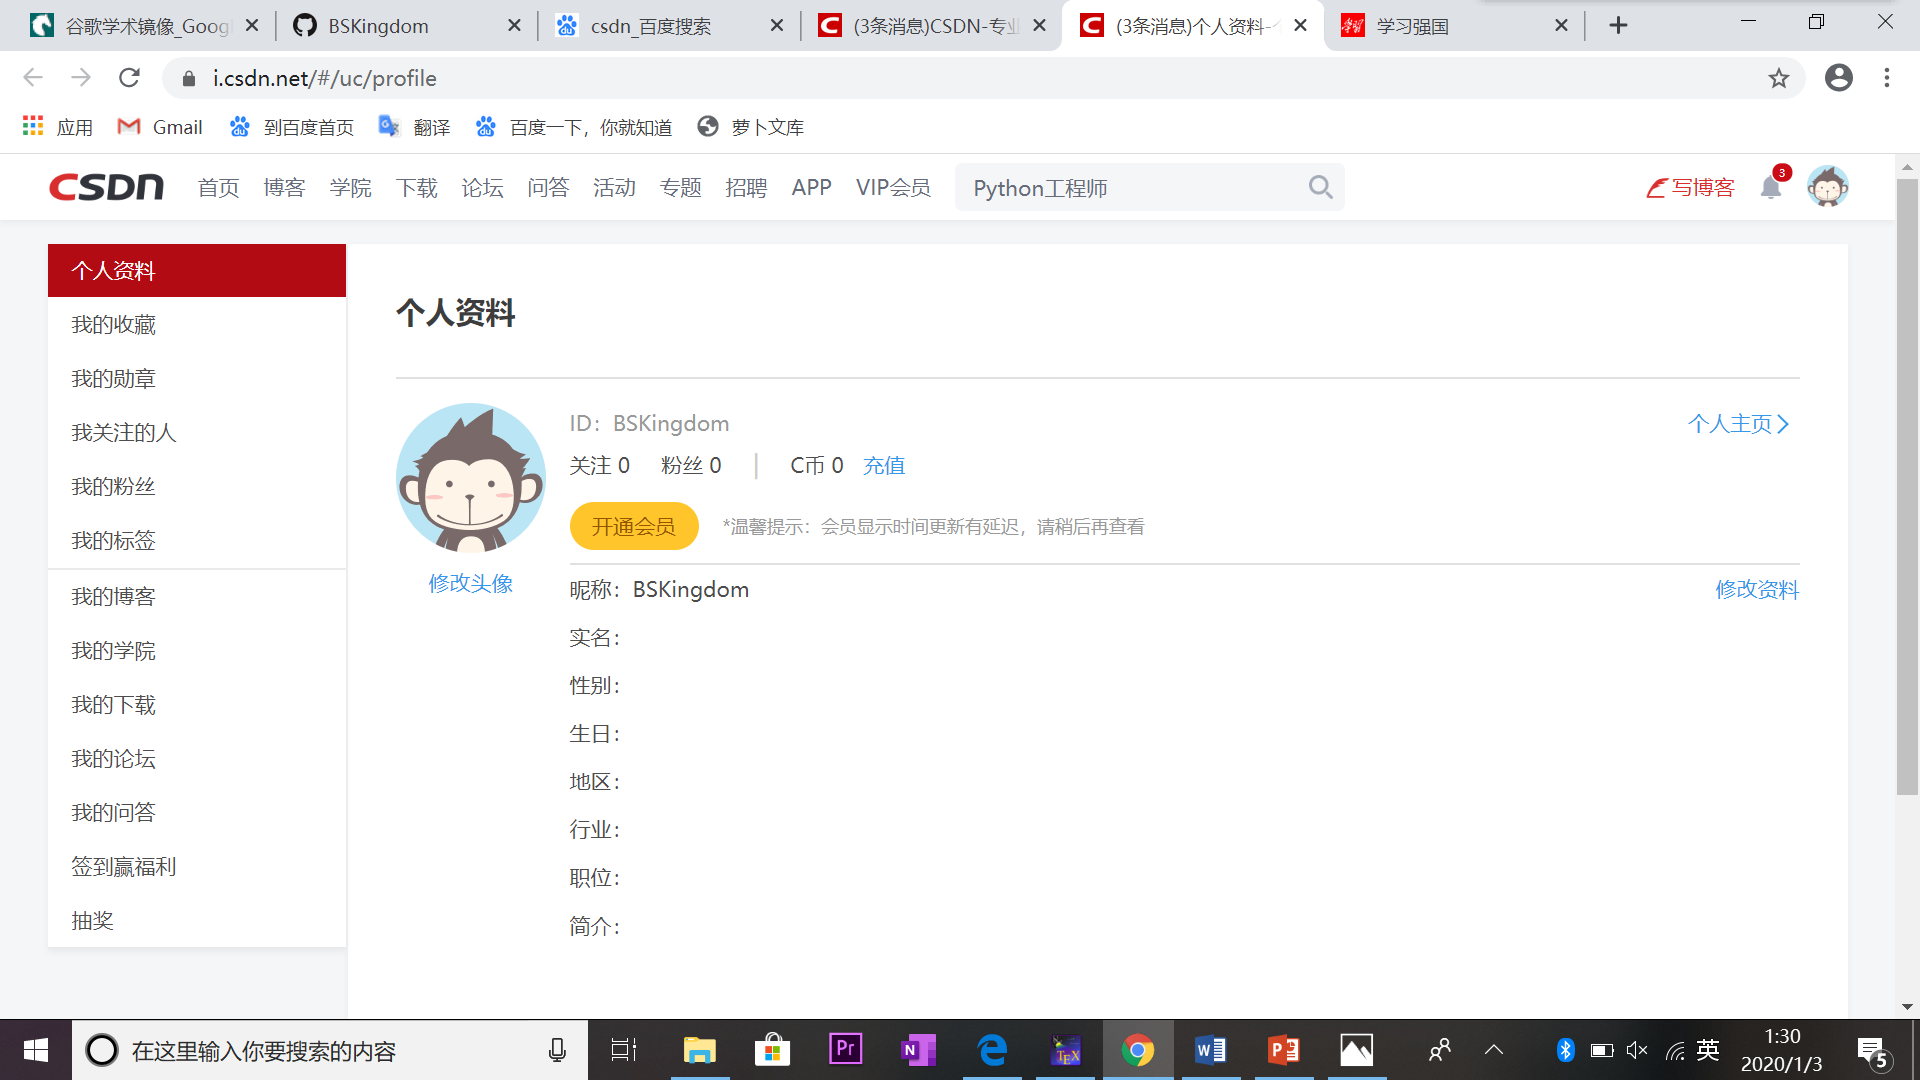
\includegraphics[width=10cm]{2020-01-03 (3).png}
    	\label{figupc}
    	
    \end{figure}
   \begin{figure}[H]
	\centering
	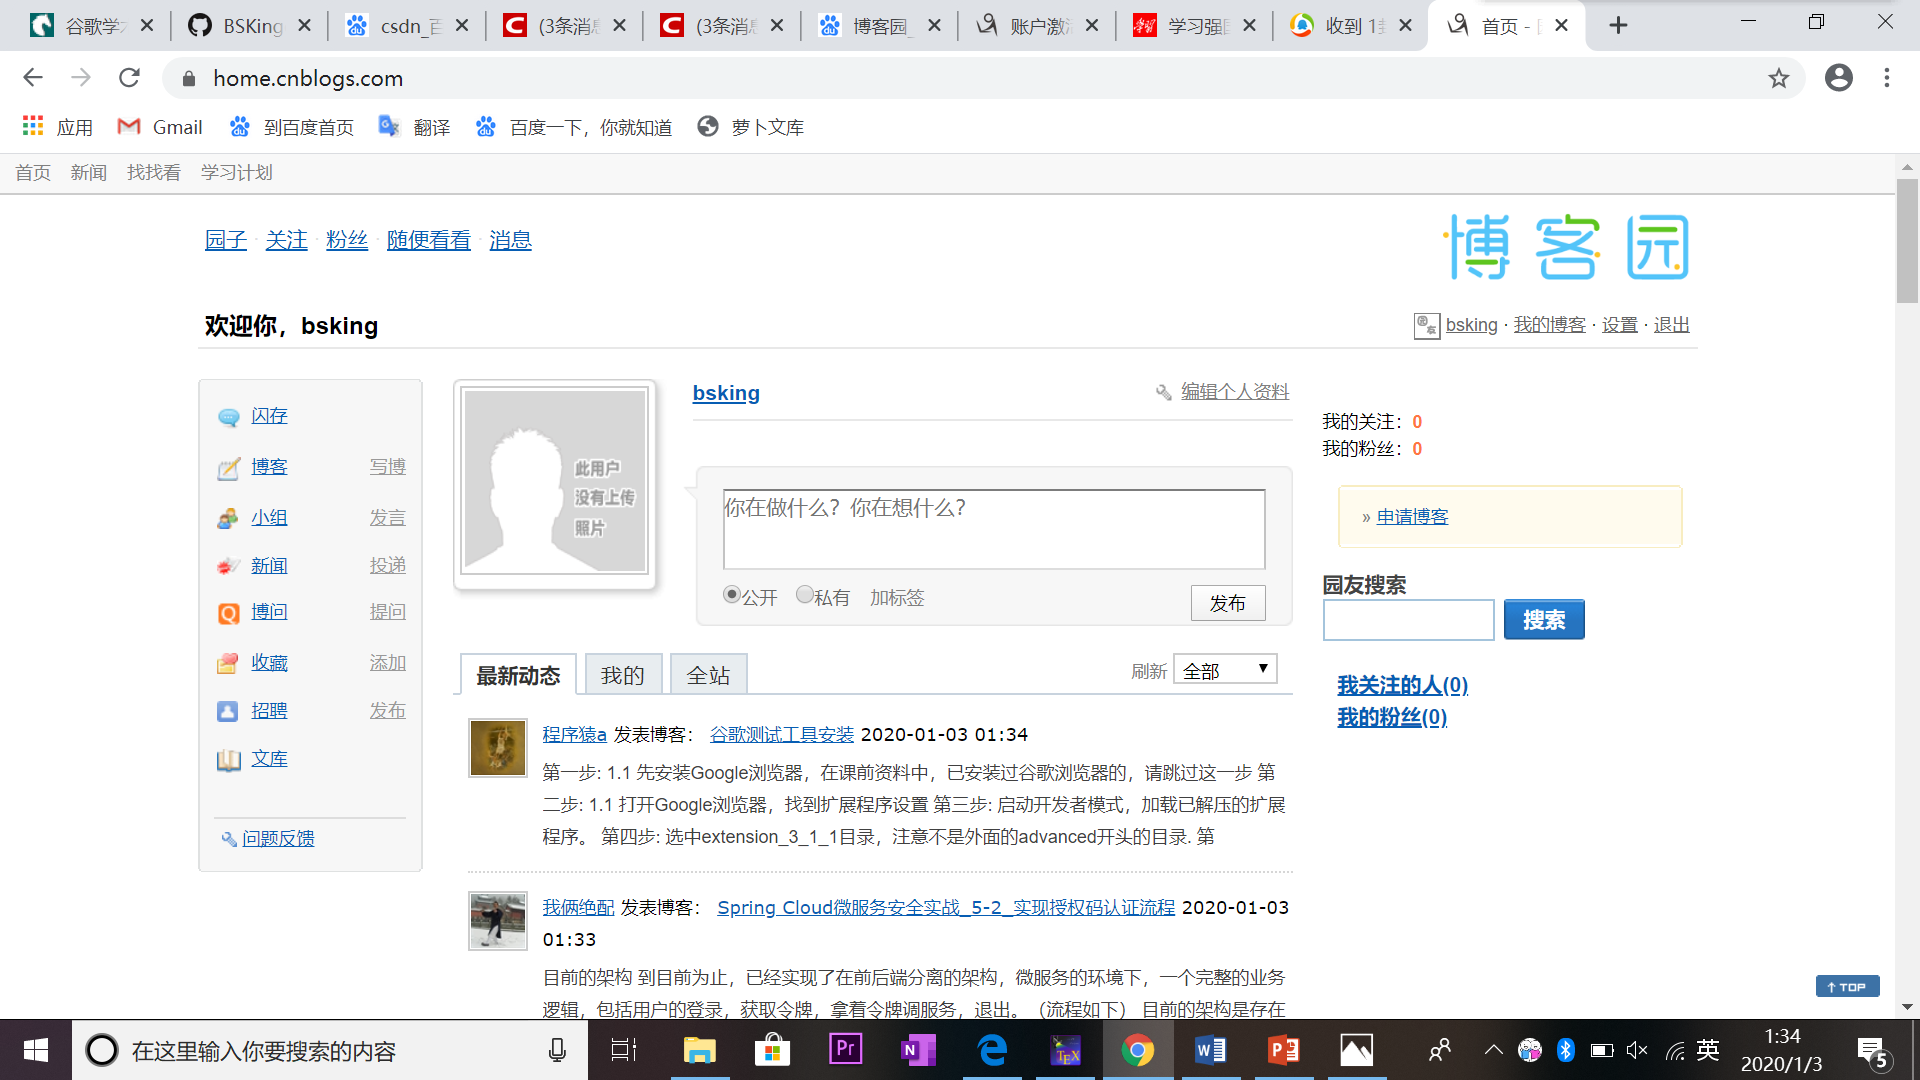
\includegraphics[width=10cm]{2020-01-03 (4).png}
	\label{figupc}
	
\end{figure}
\item
小木虫网址:http://muchong.com/bbs/space.php?uid=20375731

      \begin{figure}[H]
    	\centering
    	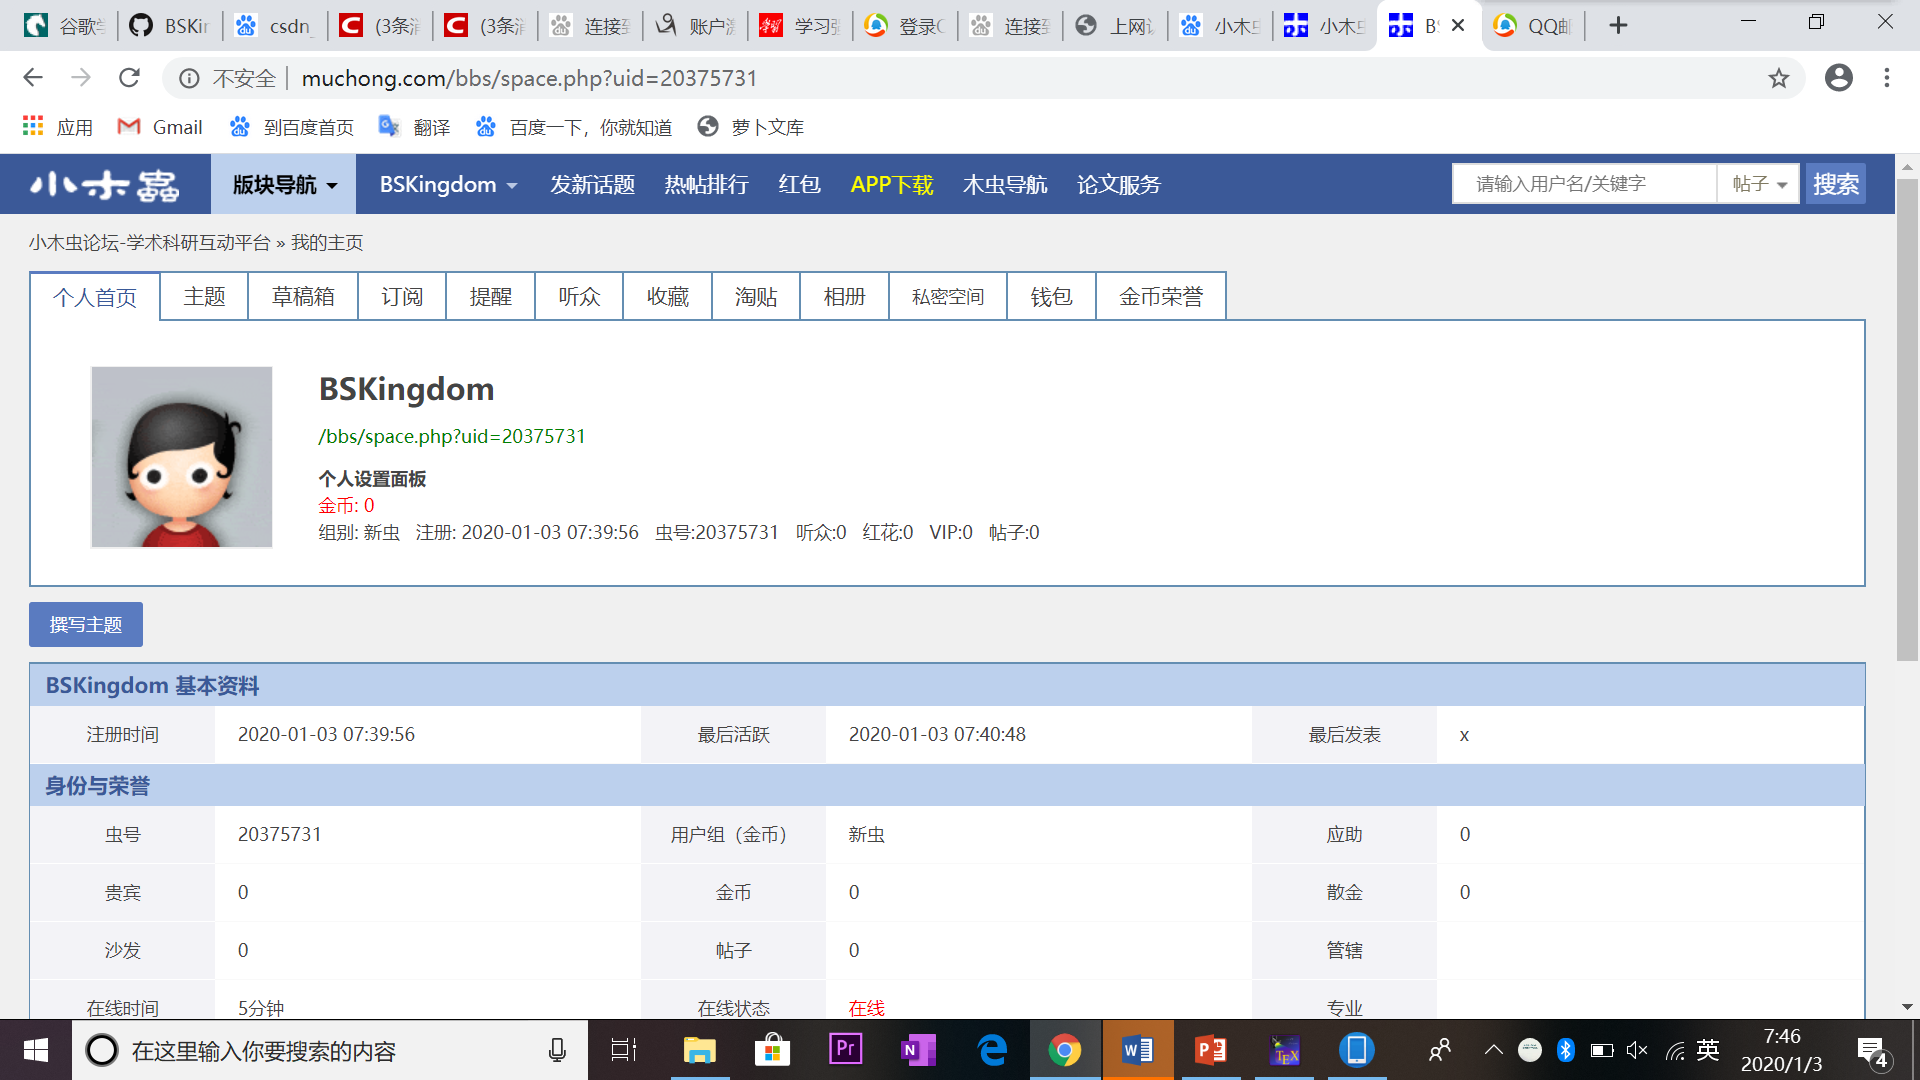
\includegraphics[width=10cm]{2020-01-03 (5).png}
    	\label{figupc}
    	
    \end{figure}
\end{itemize}


\hspace*{\fill} \\
\bibliographystyle{plain}
\bibliography{references}
\end{document}


